\chapter{Orthogonality}

\subsection*{Section~\protect{\ref{S:orthonormal}} Orthonormal Bases}
\rhead{S:orthonormal}{ORTHONORMAL BASES}

\exer{c7.4.1}
\ans The vectors $w_1 = \frac{1}{\sqrt{3}}(1,1,-1)$ and
$w_2 = \frac{1}{\sqrt{2}}(0,1,1)$ form an orthonormal basis
for the solution set.

\soln Find one vector which is a solution to the equation, for
example $(1,1,-1)$.  Then, divide the vector by its length, obtaining
the unit vector $w_1$.  By inspection, find a vector $v_2$ which
satisfies both the given equation and $w_1 \cdot v_2 = 0$.  Then set
$w_2 = \frac{1}{||v_2||}v_2$.



\subsection*{Section~\protect{\ref{S:LSA}} Least Squares Approximations}
\rhead{S:LSA}{LEAST SQUARES APPROXIMATIONS}

\exer{c7.5.1}
\ans The vectors $v_1 = \frac{1}{5}(3,4)$ and $v_2 = \frac{1}{5}(-4,3)$
form an orthonormal basis for $\R^2$.

\soln Find these vectors using Gram-Schmidt orthonormalization
(Theorem~\ref{T:orthobasis}).  More
specifically, calculate $v_1$ and $v_2$ such that:
\[
\begin{array}{rcl}
v_1 & = & \frac{1}{||w_1||}w_1 = \frac{1}{5}(3,4). \\
v_2' & = & w_2 - (w_2 \cdot v_1)v_1 = (1,5) - \frac{23}{25}(3,4)
= \frac{1}{25}(-44,33). \\
v_2 & = & \frac{1}{||v_2'||}v_2' = \frac{5}{11}
\left(\frac{1}{25}(-44,33)\right) = \frac{1}{5}(-4,3).
\end{array}
\]

\exer{c7.5.3}
By Corollary~\ref{c:extendindependent},
a linearly independent subset of $\R^n$ can be extended to form a
basis for $\R^n$ by adding linearly independent vectors
$v_{k+1},\ldots,v_n$ which are not in the span of
$\{w_1,\ldots,w_k\}$.  Then, Gram-Schmidt orthonormalization
(Theorem~\ref{T:orthobasis}) can be used
to form the orthonormal basis $\{w_1,\ldots,w_n\}$ from the basis
$\{w_1,\ldots,w_k,v_{k+1},\ldots,v_n\}$.



\subsection*{Section~\protect{\ref{S:7.6}} Least Squares Fitting of Data}
\rhead{S:7.6}{LEAST SQUARES FITTING OF DATA}

\exer{c7.6.1}
(a) \ans The best linear fit to the data is obtained with $m \approx
0.4084$ and $b \approx 0.9603$, where $m$ and $b$ are measured in
billions.

\soln Create the matrix $A$ whose columns are $w_1$ and $w_2$.  Then use
\Ref{E:nearestvector} to compute the best values for $m$ and $b$.

(b) In 1910, $P \approx 408.4(1) + 960.3 = 1369$ million people.

\para In 2000, $P \approx 408.4(10) + 960.3 = 5044$ million people.

(c) \ans The prediction for 2000 is likely to be low.

\soln As shown in Figure~\ref{c7.6.1}, a linear approximation does not
fit the data points well.  To understand why, assume that population
change is governed by the differential equation:
\[
\frac{dP}{dT} = rP
\]
where $r$ is constant.  Then $\frac{d^2P}{dT^2} = r^2P > 0$.
Then the population curve is concave up, and a linear approximation
underestimates the population at the endpoints of the curve.

\begin{figure}[htb]
		\centerline{%
		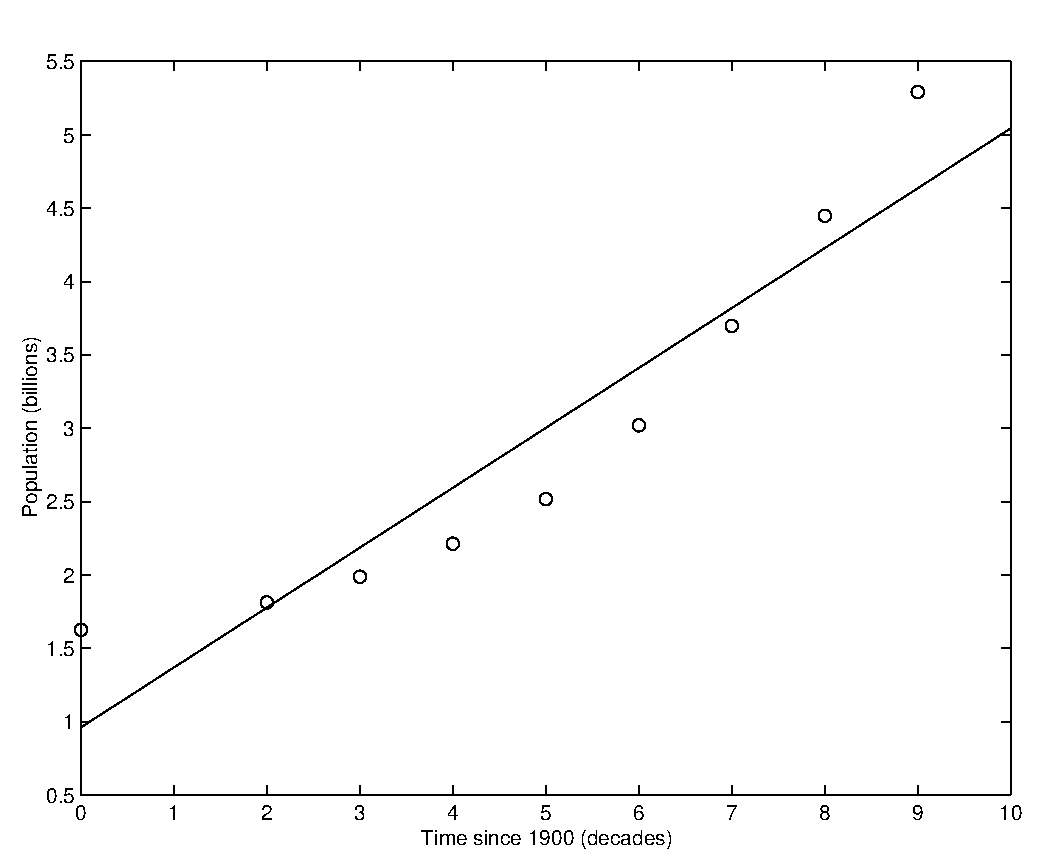
\psfig{file=exfigure/7-6-1.eps,width=3.0in}}
	\exercap{c7.6.1}
\end{figure}

\exer{c7.6.3}
\ans Let $R$ be the number of days in the year with precipitation and
let $s$ be the percentage of sunny hours to daylight hours.  Then the
best linear estimate of the relationship between the two is:
\[ R \approx 199.2 - 156.6s. \]

\soln In \Matlabp, enter the data for number of rainy days as the vector
$R$, and then enter the data for percentage of sunny hours as the vector
$s_1$.  Then create the $1 \times 10$ vector $s_2 = (1,1,\dots,1)$.  Now,
find the best vector $b = (b_1,b_2)$ such that $R = b_1s_1 + b_2s_2$. 
This vector can be found using \Ref{E:nearestvector}.  The solution vector
is $(b_1,b_2) \approx (-156.6,199.2)$.  Figure~\ref{c7.6.3} shows the
actual data graphed against the linear estimate.

\begin{figure}[htb]
		\centerline{%
		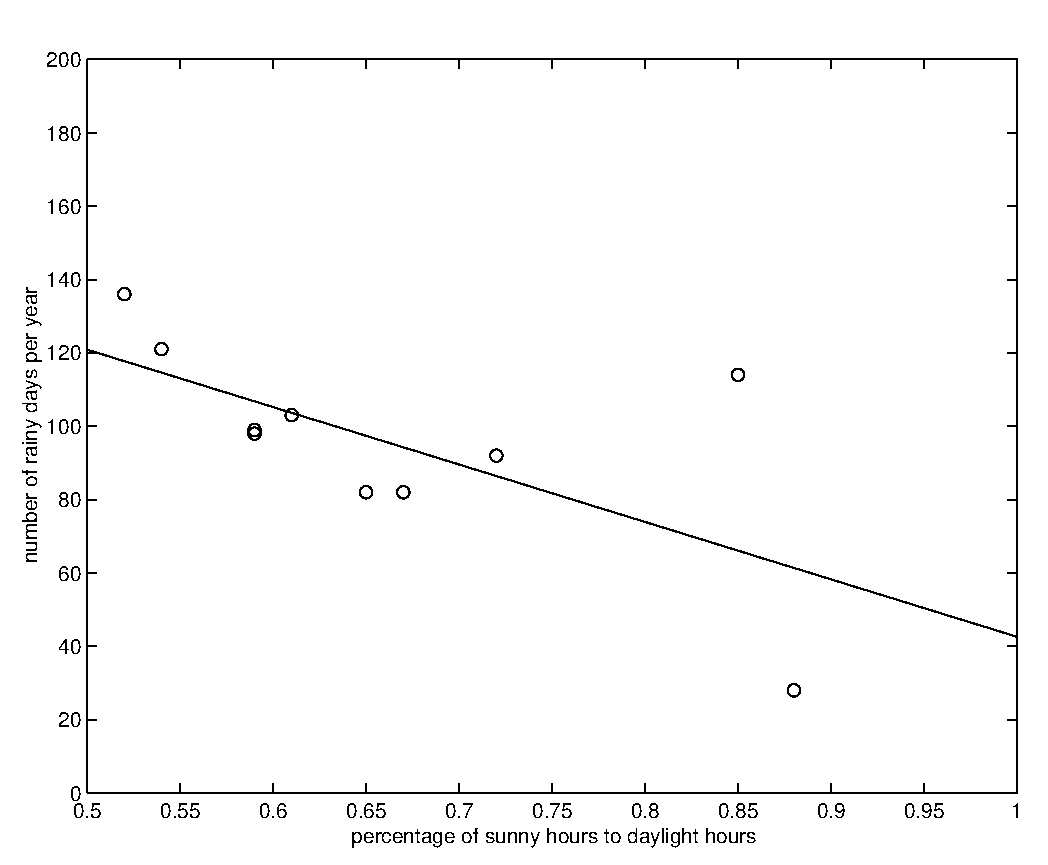
\psfig{file=exfigure/7-6-3.eps,width=3.0in}}
	\exercap{c7.6.3}
\end{figure}



\newpage
\subsection*{Section~\protect{\ref{S:symmetric}} Symmetric Matrices}
\rhead{S:symmetric}{SYMMETRIC MATRICES}

\exer{c7.7.1}
(a) We can calculate the discriminant $D$ of matrix $A$ using
\Ref{e:discriminant}:
\[ D = \trace(A)^2 - 4\det(A) = (a + d)^2 - 4(ad - b^2) =
a^2 + 2ad + b^2 - 4ad + 4b^2 = (a - d)^2 + 4b^2. \]
Therefore, $D \geq 0$ for all real symmetric matrices $A$.  The
eigenvalues of $A$ are
\[ \lambda_1 = \frac{(a + d) + \sqrt{D}}{2} \AND
\lambda_2 = \frac{(a + d) - \sqrt{D}}{2}. \]
Thus, $\lambda_1$ and $\lambda_2$ are real since $D$ is non-negative.

(b) Matrix $A$ has equal eigenvalues only if $D = 0$.  According to
the computation in (a) of this problem, $D = 0$ only if $a = d$ and
$b = 0$.  Therefore, if $\lambda_1 = \lambda_2$, then $A$ is a
multiple of $I_2$.

\exer{exer:powita}
\ans The eigenvectors of $A$ are $w_1 = (1,1)$ and
$w_2 = (1,-1)$ with eigenvalues $\lambda_1 = 4$ and $\lambda_2 = -2$.  

\soln Note that any matrix of the form $\mattwo{a}{b}{b}{a}$
has eigenvectors $w_1$ and $w_2$ with eigenvalues
$\lambda_1 = a + b$ and $\lambda_2 = a - b$.
By iterating using {\tt map}, we see that $v_j$ approaches a multiple
of $(1,1)$ as $j$ increases for $v_0 \neq (1,-1)$.  If $v_0$ is a
multiple of $(1,-1)$, then $v_j$ is a multiple of $(1,-1)$ for all $j$.

\para In Exercises~\ref{exer:powita} -- \ref{exer:powitc} let $u_1$ be the
eigenvector of matrix associated to the eigenvalue $\lambda_1$ where
$|\lambda_1| > |\lambda_2|$. These exercises demonstrate that $v_j$ 
approaches the direction of $u_1$ as $j$ increases when $v_0$ is
not a scalar multiple of $u_2$.

\exer{exer:powitc}
\ans The eigenvectors of $C$ are $w_1 = (1,1)$ and $w_2 = (1,-1)$ with 
eigenvalues $\lambda_1 = -2$ and $\lambda_2 = 2.01$.  

\soln See comment after the solution to Exercise~\ref{exer:powita}.
By iterating using {\tt map}, we see that $v_j$ approaches a multiple
of $(1,-1)$ as $j$ increases for $v_0 \neq (1,1)$.  If $v_0$ is a
multiple of $(1,1)$, then $v_j$ is a multiple of $(1,1)$ for all $j$.



\subsection*{Section~\protect{\ref{S:QR}} Orthogonal Matrices and $QR$
Decomposition}
\rhead{S:QR}{ORTHOGONAL MATRICES AND $QR$ DECOMPOSITION}

\exer{c7.9.1a} \ans The matrix is not orthogonal.

\soln By Lemma~\ref{lem:orthprop}, a matrix
$A$ is orthogonal if and only if $A^tA = I_n$.
\[
\mattwo{2}{0}{0}{1}\mattwo{2}{0}{0}{1} = \mattwo{4}{0}{0}{1} \neq I_2.
\]

\exer{c7.9.1c} The matrix is orthogonal, since
\[
\matthree{0}{0}{-1}{-1}{0}{0}{0}{1}{0}
\matthree{0}{1}{0}{0}{0}{-1}{-1}{0}{0} =
I_3.
\]

\exer{c7.9.1e} The matrix is not orthogonal, since all orthogonal matrices
are square.

\exer{c7.9.3a}
$H = I_2 - \frac{2}{2}\vectwo{1}{1}\left(\begin{array}{rr} 1 & 1
\end{array}\right) = \mattwo{1}{0}{0}{1} - \mattwo{1}{1}{1}{1}
= \mattwo{0}{-1}{-1}{0}.$

\exer{c7.9.3c}
$H = I_3 - \frac{2}{27}\matthree{1}{-1}{-5}{-1}{1}{5}{-5}{5}{25}
= \frac{1}{27}\matthree{25}{2}{10}{2}{25}{-10}{10}{-10}{-50}$.

\exer{c7.9.4}
\ans The matrix that reflects the plane across $(1,2)$ is
\[
H = \mattwo{-\frac{3}{5}}{\frac{4}{5}}{\frac{4}{5}}{\frac{3}{5}}.
\]

\soln The matrix that reflects the plane across $(1,2)$ is the
Householder matrix associated to the vector $u$, where $u \cdot (1,2)
= 0$.  Compute $H$, the Householder matrix associated to $u = (2,-1)$.

\exer{c7.5.5a}
The orthonormal basis generated by the command {\tt [Q R] = qr(A,0)} is:
\begin{verbatim}
v1 =          v2 =
   -0.7071        0.7071
    0.7071        0.7071
\end{verbatim}

\newpage
\exer{c7.5.5c}
The orthonormal basis generated by the command {\tt [Q R] = qr(A,0)} is:
\begin{verbatim}
v1 =          v2 =          v3 = 
   -0.2673        0.0514       -0.9623
    0.5345       -0.8230       -0.1925
   -0.8018       -0.5658        0.1925
\end{verbatim}

\exer{c7.5.6}
\ans
\begin{verbatim}
H1 =                                   H2 =
   0.6245  -0.7220  -0.2744   0.1155      0.2807   0.6679  -0.3083  -0.6165
  -0.7220  -0.3885  -0.5276   0.2222      0.6679   0.3798   0.2862   0.5725
  -0.2744  -0.5276   0.7995   0.0844     -0.3083   0.2862   0.8679  -0.2642
   0.1155   0.2222   0.0844   0.9645     -0.6165   0.5725  -0.2642   0.4716

H =
   -0.2935    0.1305   -0.6678   -0.6714
   -0.4365   -0.6536   -0.4053    0.4669
   -0.7279   -0.1065    0.6051   -0.3043
   -0.4398    0.7378   -0.1536    0.4885
\end{verbatim}

\soln Find $H_1$ in \Matlab by typing
\begin{verbatim}
H1 = eye(4) - 2/(u1'*u1)*u1*u1'
\end{verbatim}

Calculate $H_2$ similarly.  Confirm that $H = H_1H_2$ is orthogonal by
computing the product $H^tH$ to see that it is $I_4$.
